\documentclass[10pt,a4paper]{article}
\usepackage[utf8]{inputenc}
\usepackage{amsmath}
\usepackage{gensymb}
\usepackage{amsfonts}
\usepackage{siunitx}
\usepackage[european]{circuitikz}
\usepackage{geometry}
\newgeometry{tmargin=2cm, bmargin=2cm, lmargin=2cm, rmargin=2cm}
\usepackage{amssymb}
\usepackage{multirow}
\usepackage{polski}
\usepackage{graphicx}
\author{\textbf{T. Fąs}}
\title{\textbf{ZAWARTOŚĆ IZOTOPU $^{40}$K W POTASIE NATURALNYM}}
\begin{document}
\maketitle

\begin{center}
\textbf{\subsection*{STRESZCZENIE}}
\end{center}
W doświadczeniu wyznaczono zawartość procentową $p$ radioizotopu $^{40}$K w solach potasu K$_{2}$CO$_{3}$. Otrzymano wartość $s=(0,0203\pm0,0012) \%$. Wartość ta jest prawie dwukrotnie wyższa od oczekiwanej, prawdopodobnie na skutek błędnie działającej aparatury. Oprócz tego określono energetyczną zdolność rozdzielczą spektrometru, która wynosi około $9\%$.    


\begin{center}
\textbf{\subsection*{WSTĘP}}
\end{center}
W środowisku naturalnym występują trzy izotopy potasu: $^{39}$K, $^{40}$K i $^{41}$K, z czego tylko $^{40}$K jest radioaktywny. W 89$\%$ przypadków ulega on rozpadowi $\beta^{-}$. W pozostałych 11$\%$ przypadków dochodzi do emisji kwantu $\gamma$. W doświadczeniu mierzono liczbę rozpadów $\gamma$ w czasie 30 minut i na tej podstawie wyznaczono stosunek masy $^{40}$K do całości naturalnie występującego potasu. 

Jeśli w czasie $t$ odnotowano $N$ rozpadów, to z prawa zaniku promieniotwórczego można wyznaczyć początkową liczbę $N_{0}$ jąder $^{40}$K. Relacją między $N$ i $N_{0}$ dana jest następującym wzorem:
\begin{equation}
N=N_{0}\left(1-e^{-\lambda t} \right),
\end{equation}
gdzie $\lambda$ jest stałą rozpadu. Znając czas połowicznego zaniku $T_{1/2}=1,26\cdot10^9$ lat można go powiązać z wartością $\lambda$ następującą relacją:
\begin{equation}
\lambda=\dfrac{\ln 2}{T_{1/2}}.
\end{equation}

Znając masy molowe $^{39}$K i $^{40}$K oznaczone kolejno $m_{39}$ i $m_{40}$, całkowitą masę $M$ próbki soli K$_{2}$CO$_{3}$ oraz jej masę molową $m_{s}$ można wyznaczyć:

masę potasu $^{40}$K ze wzoru:
\begin{equation}
M_{40}=\dfrac{N_{0}}{N_{A}}m_{40},
\end{equation}
gdzie $N_{A}$ jest liczą Avogadra; masę $^{39}$K ze wzoru:
\begin{equation}
M_{39}=\left(\dfrac{2M}{m_{s}}-\dfrac{N_{0}}{N_{A}}\right)m_{39}
\end{equation}
oraz szukany stosunek $s=M_{40}/(M_{39}+M_{40})$.
\begin{center}
\textbf{\subsection*{UKŁAD DOŚWIADCZALNY}}
\end{center}
Układ doświadczalny składał się ze spektrometru podłączonego do komputera, próbki cezu $^{137}$Cs, kobaltu $^{60}$Co oraz próbki soli K$_{2}$CO$_{3}$ o masie $M=1011,91$g. Wykonano 15-minutowy pomiar widma cezu oraz pomiar widma kobaltu, węglanu potasu i tła, z czego każdy z tych pomiarów trwał po 30 minut. Wyniki zostały zapisane w pamięci komputera.

\begin{center}
\textbf{\subsection*{WYNIKI POMIARÓW}}
\end{center}
Wyniki pomiarów w postaci wykresów widm przedstawione są na Rysunkach 1-4.

\begin{figure}[h!]
\centering
\begin{minipage}{0.5\textwidth}
  \centering
  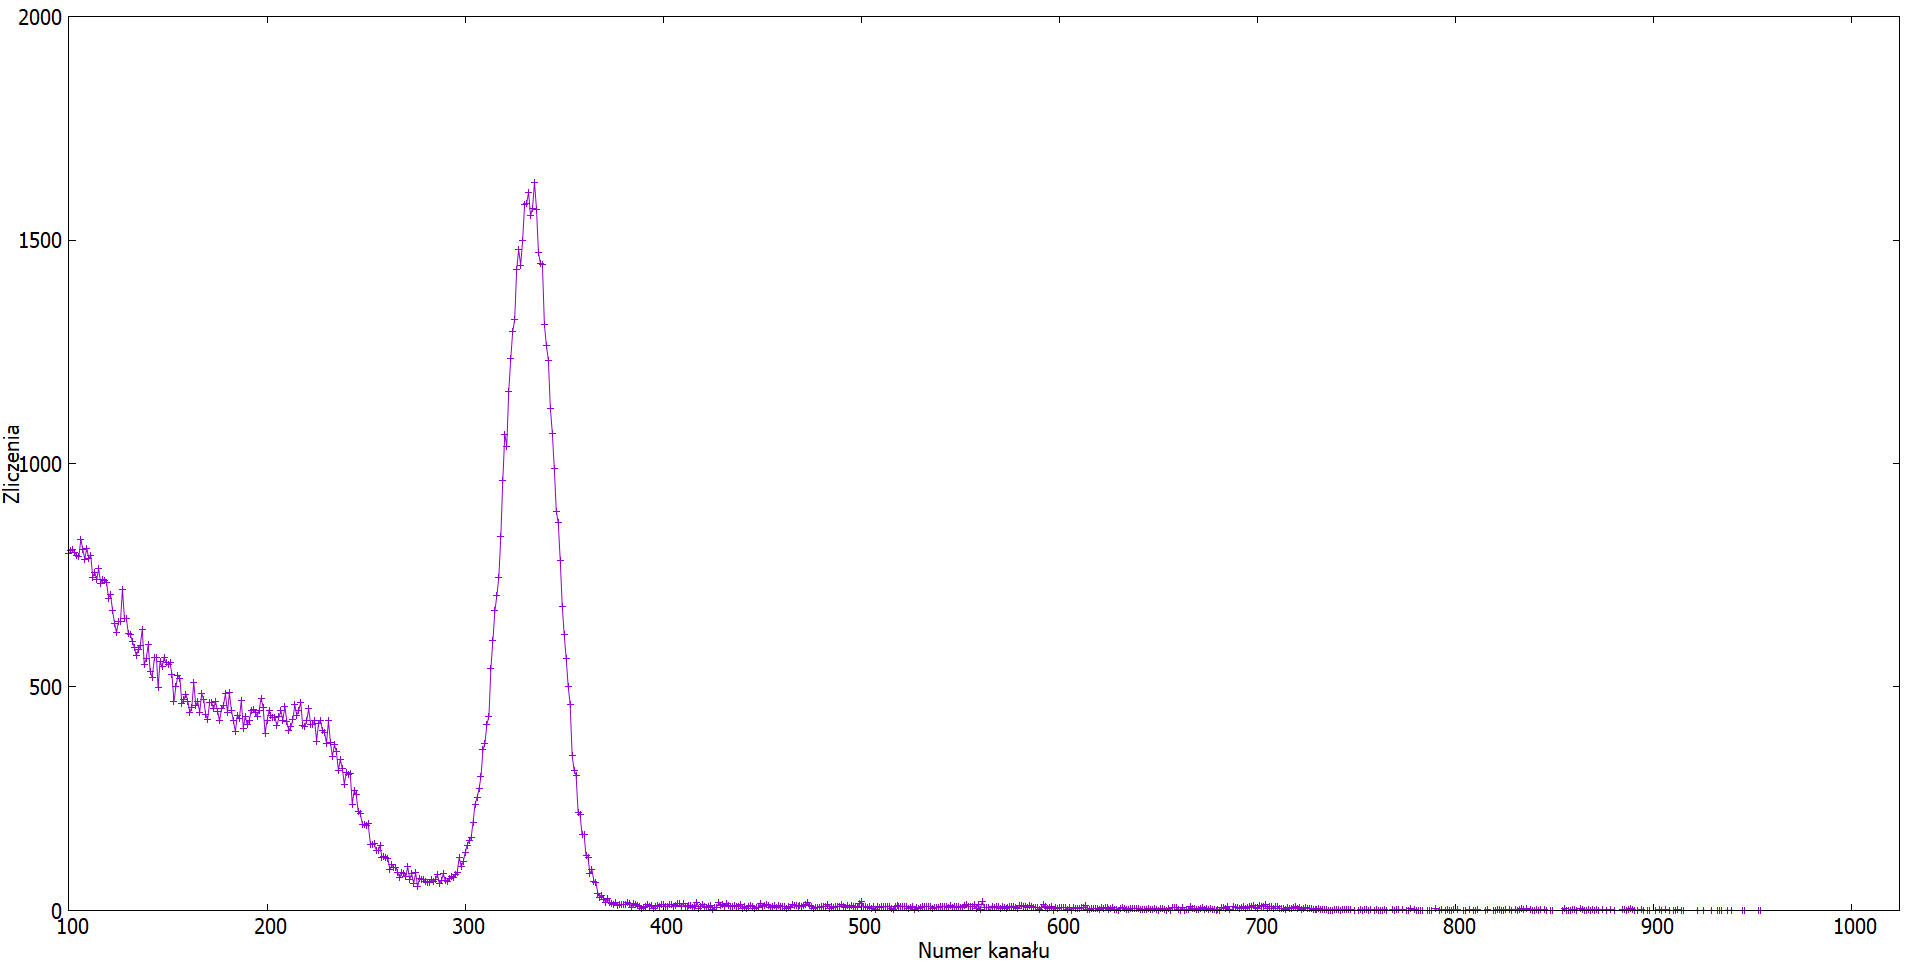
\includegraphics[width=8cm, height=5cm ]{rap14rys1} 
\caption{Widmo cezu.}
\end{minipage}%
\begin{minipage}{0.5\textwidth}
  \centering
  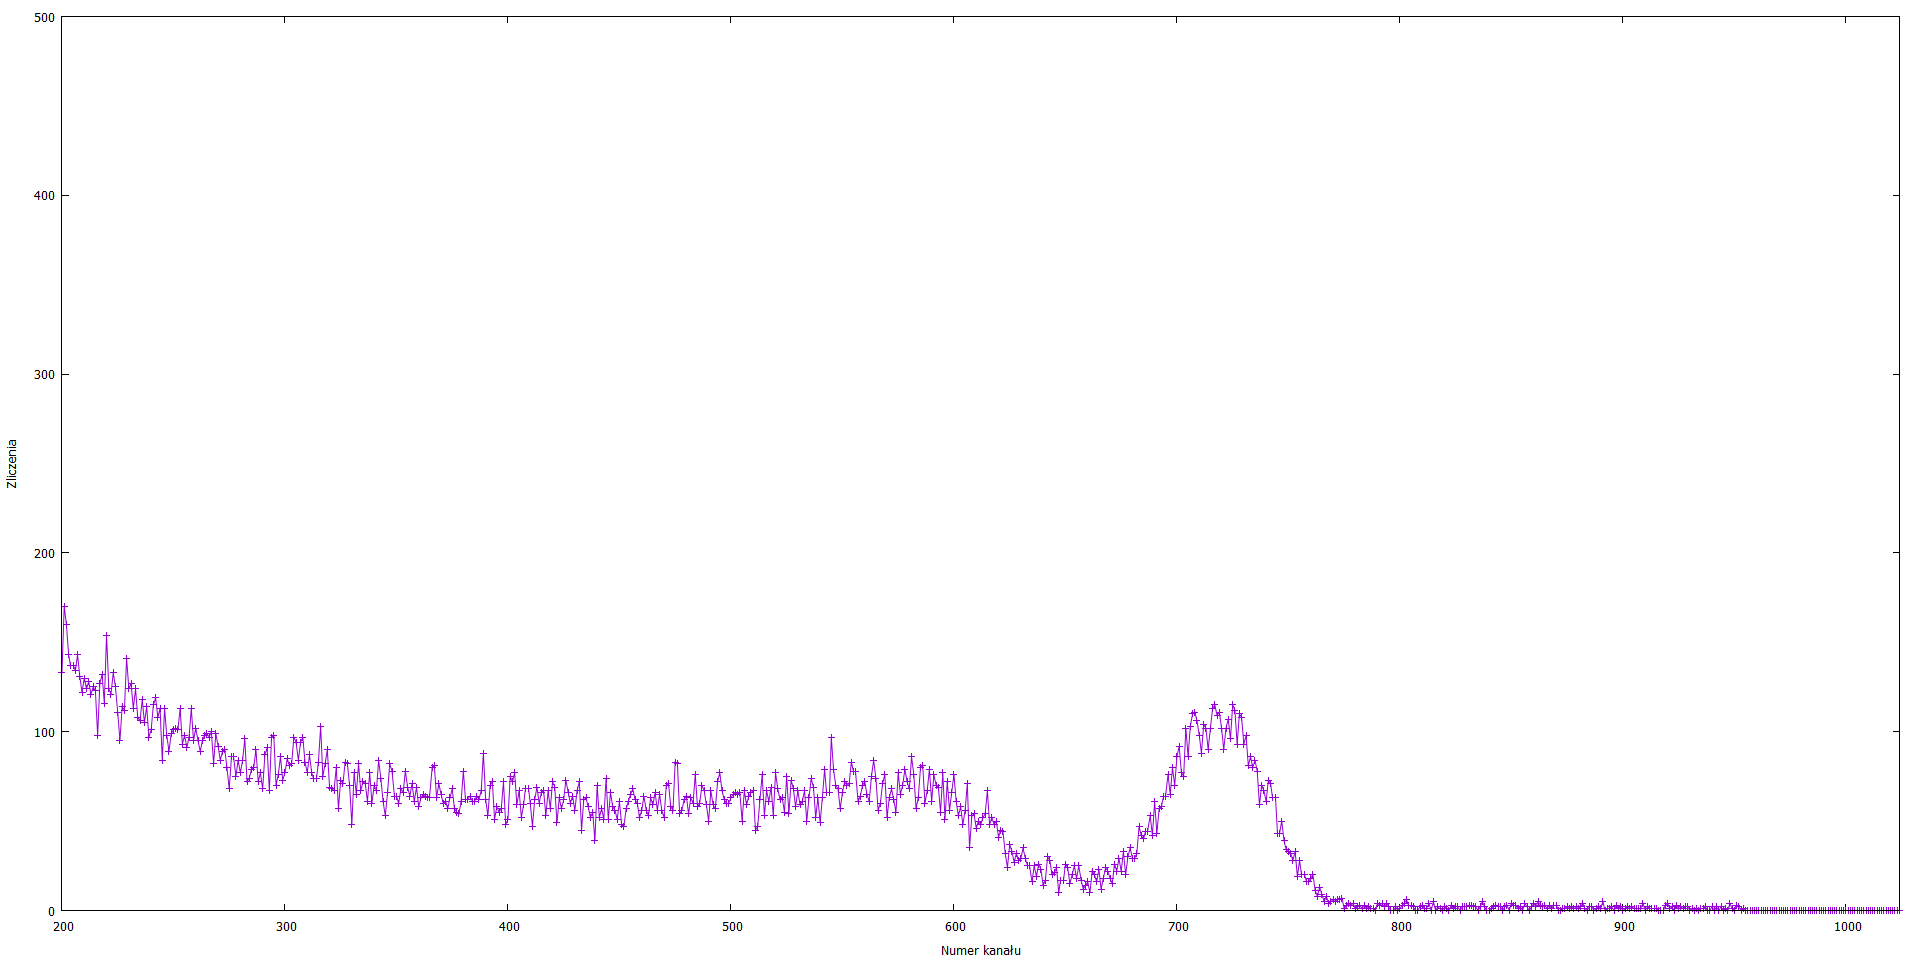
\includegraphics[width=8cm, height=5cm ]{rap14rys2} 
\caption{Widmo kobaltu.}
\end{minipage}
\end{figure}
\begin{figure}[h!]
\centering
\begin{minipage}{0.5\textwidth}
  \centering
  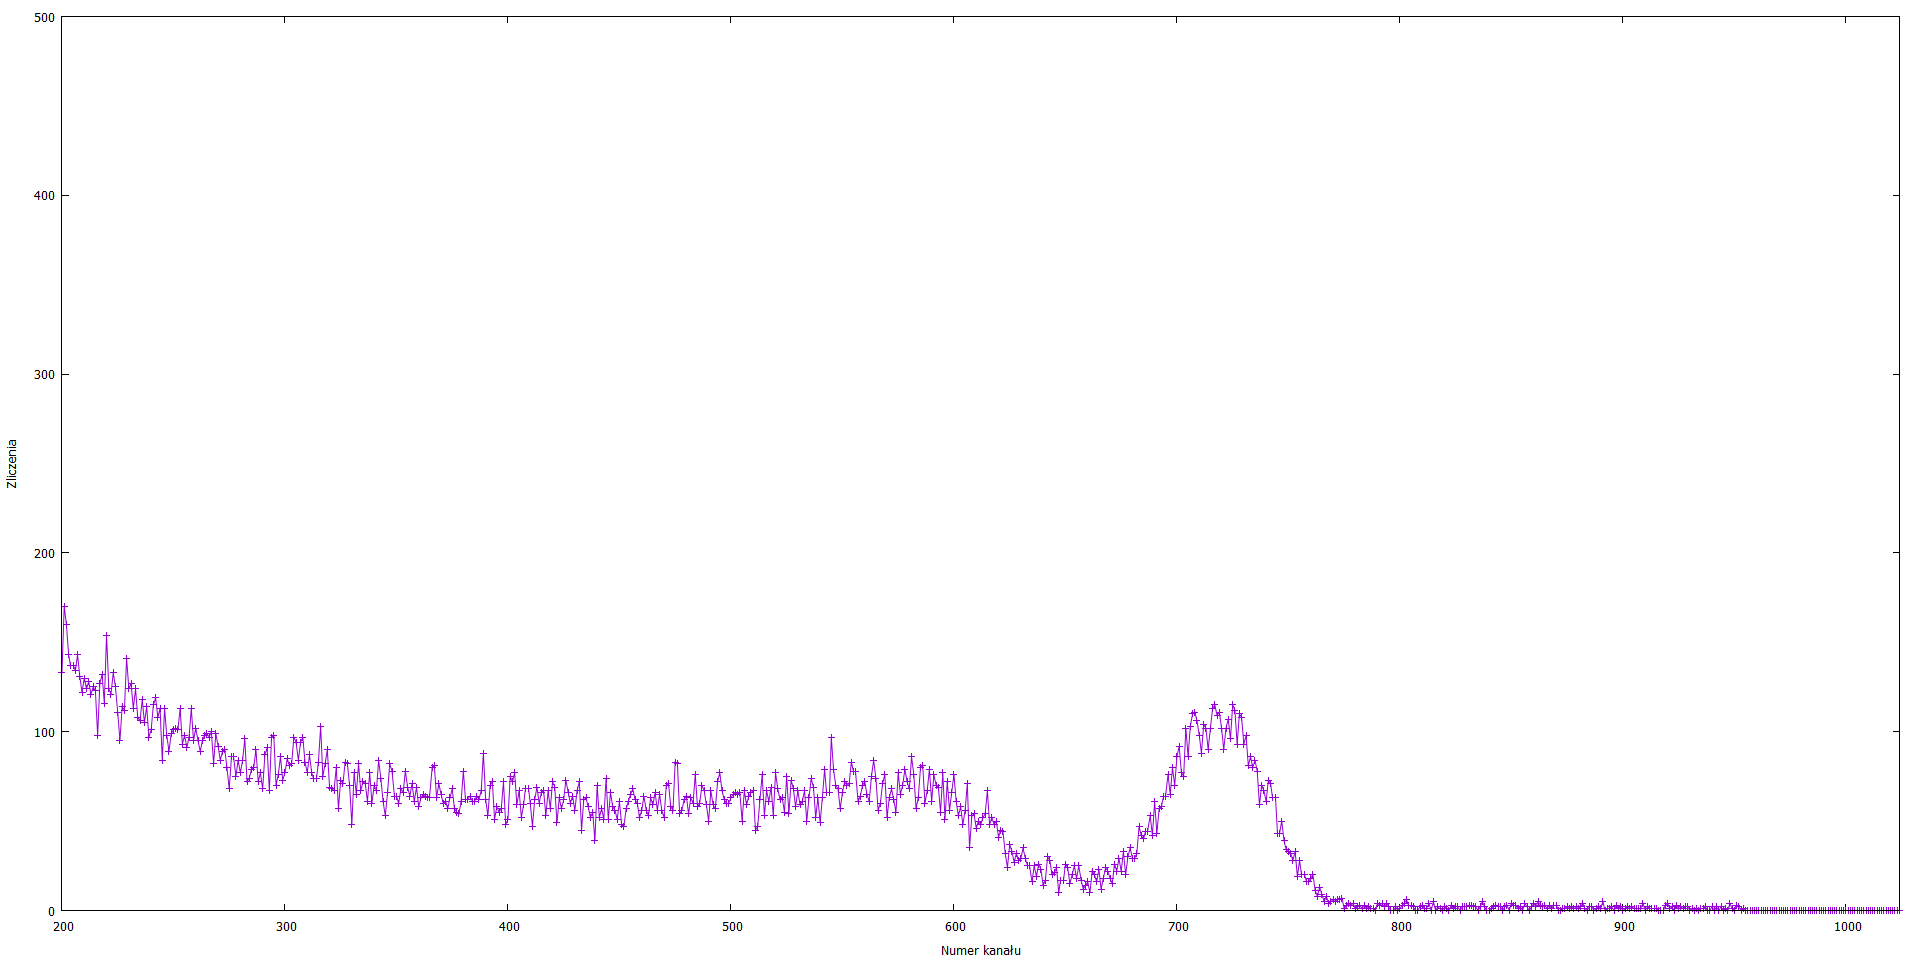
\includegraphics[width=8cm, height=5cm ]{rap14rys31} 
\caption{Widmo potasu.}
\end{minipage}%
\begin{minipage}{0.5\textwidth}
  \centering
  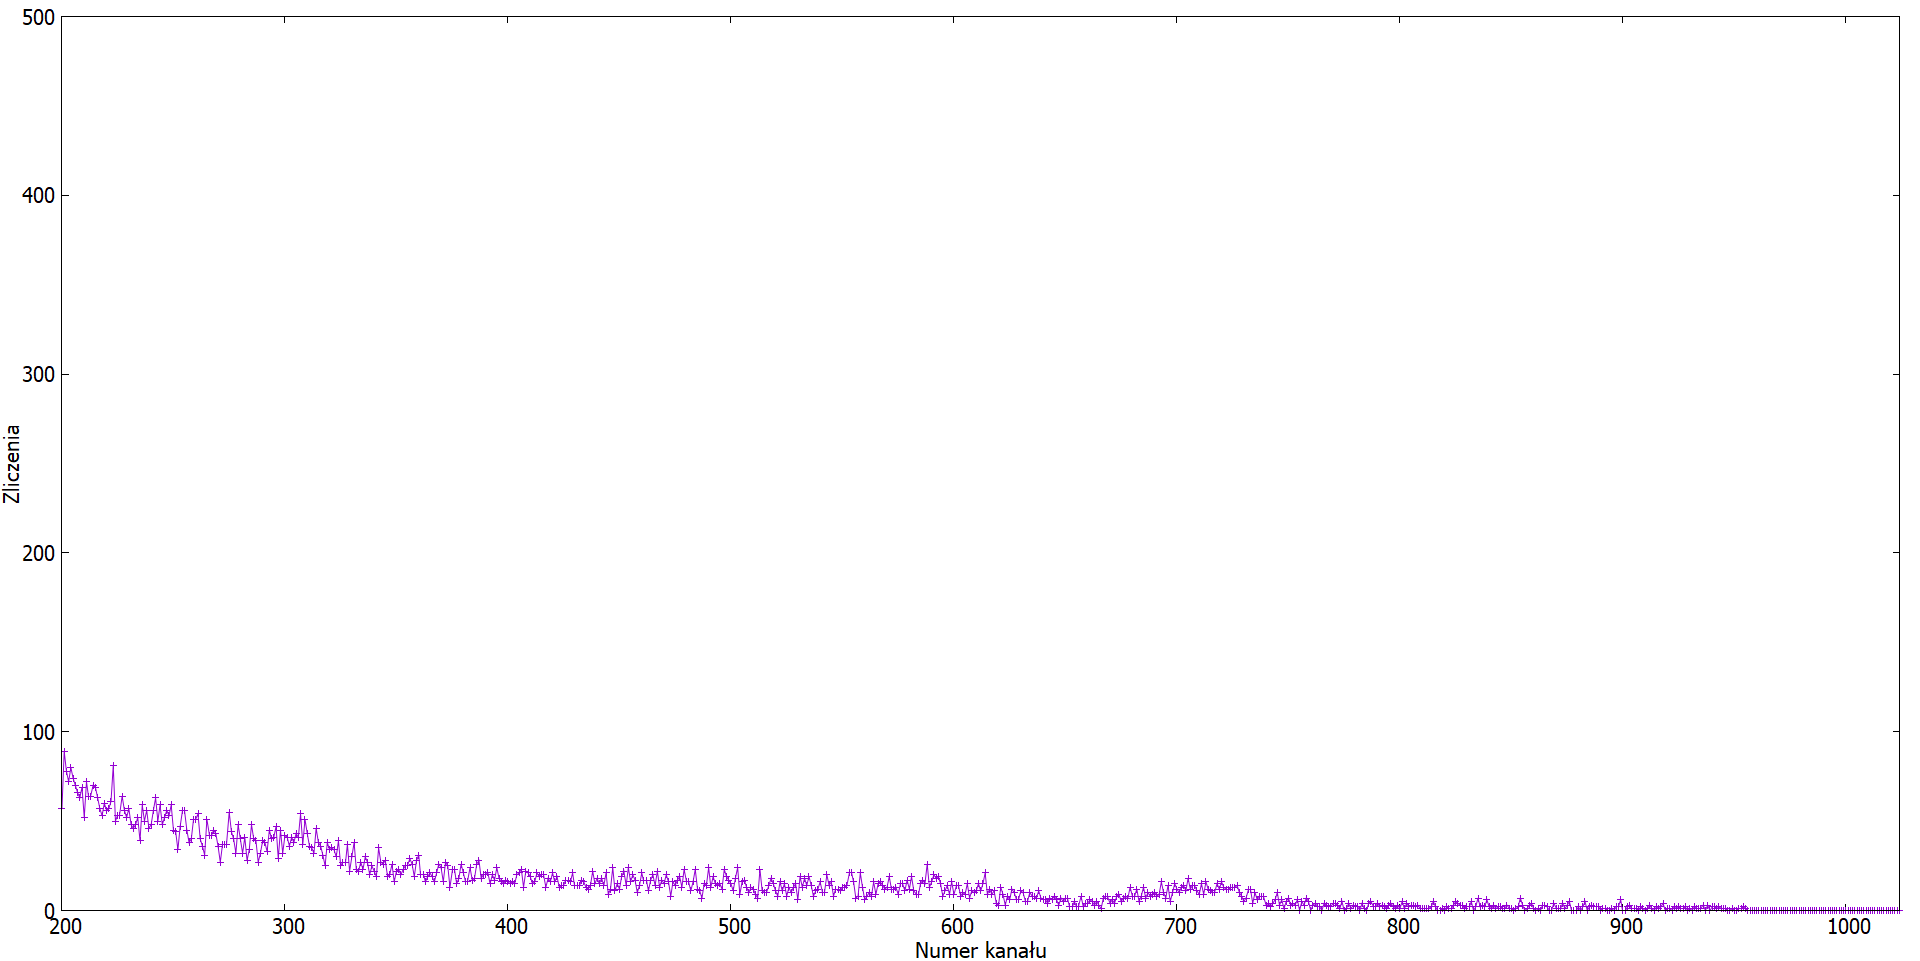
\includegraphics[width=8cm, height=5cm ]{rap14rys32} 
\caption{Widmo tła.}
\end{minipage}
\end{figure}


\begin{center}
\textbf{\subsection*{ANALIZA DANYCH}}
\end{center}
Liczba odnotowanych zliczeń podlega rozkładowi Poissona, tak więc niepewność dla $n$ zliczeń wynosi $\sqrt{n}$. W ten sposób obliczono niepewności związane z każdym z widm. 
Następnie od każdego z widm odjęto widmo tła. Niepewność tej różnicy obliczono, korzystając z metody propagacji małych błędów. Ogólny wzór przenoszenia niepewności w tej metodzie jest następujący:
 \begin{equation}
 u_{f}^2=\sum_{i=1}^n \left( \dfrac{\partial f}{\partial x_{i}}u_{i}\right)^2+\sum_{i=1, i\neq j}^n \left( \dfrac{\partial f}{\partial x_{i}}\dfrac{\partial f}{\partial x_{j}}c_{ij}\right),
 \end{equation}
 gdzie wielkość $f$ zależy od wielkości $x_{i}$ o niepewnościach $u_{i}$ i o ocenach kowariancji $c_{ij}$ \cite{tay1}.
 
 Następnie do każdego z pików przy pomocy programu \textit{gnuplot} dopasowano zależność postaci:
 \begin{equation}
 n(x)=\dfrac{N}{\sqrt{2\pi}\sigma}\exp{\left(\dfrac{-\left(x-\mu\right)^2}{2\sigma ^2}\right)},
 \end{equation}
 gdzie $x$ jest numerem kanału. Krzywe najlepszego dopasowania przedstawiono na Rysunkach 5-7. Parametry dopasowania przedstawiono w Tabeli 1.
 
 \begin{figure}[h!]
\centering
\begin{minipage}{0.5\textwidth}
  \centering
  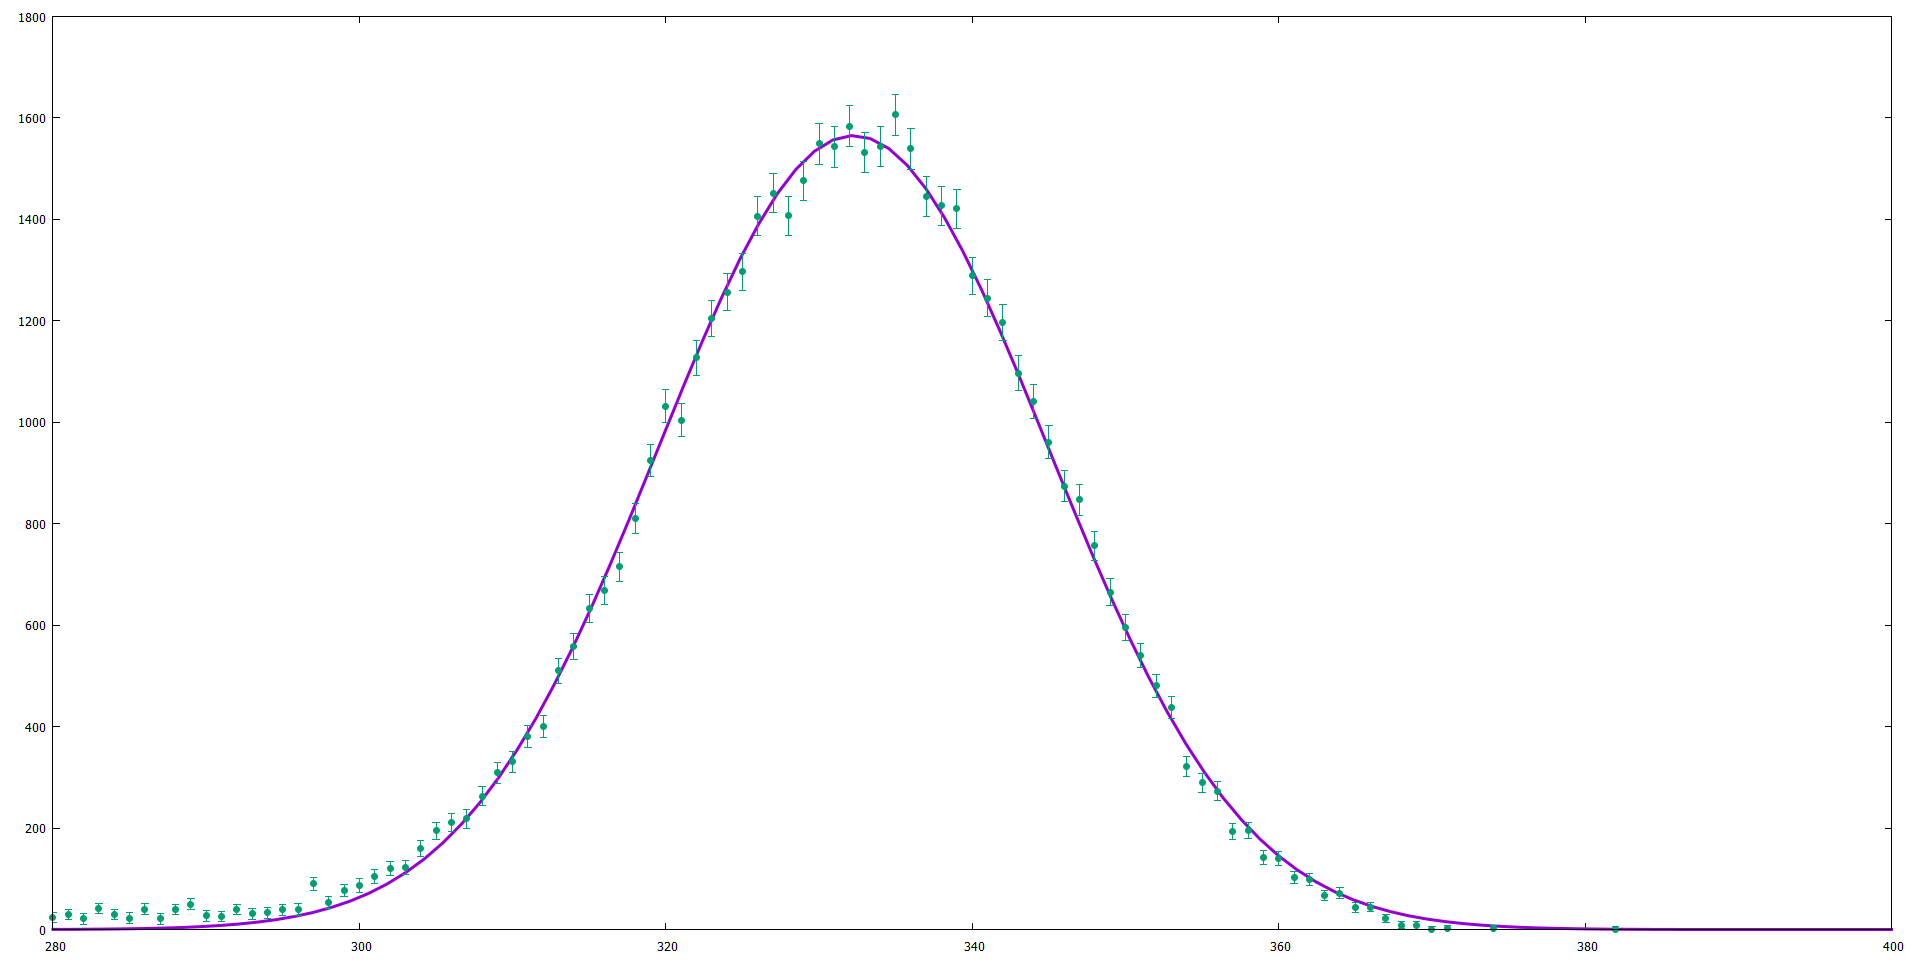
\includegraphics[width=8cm, height=5cm ]{rap14rys4} 
\caption{Krzywa dopasowania: pik cezu.}
\end{minipage}%
\begin{minipage}{0.5\textwidth}
  \centering
  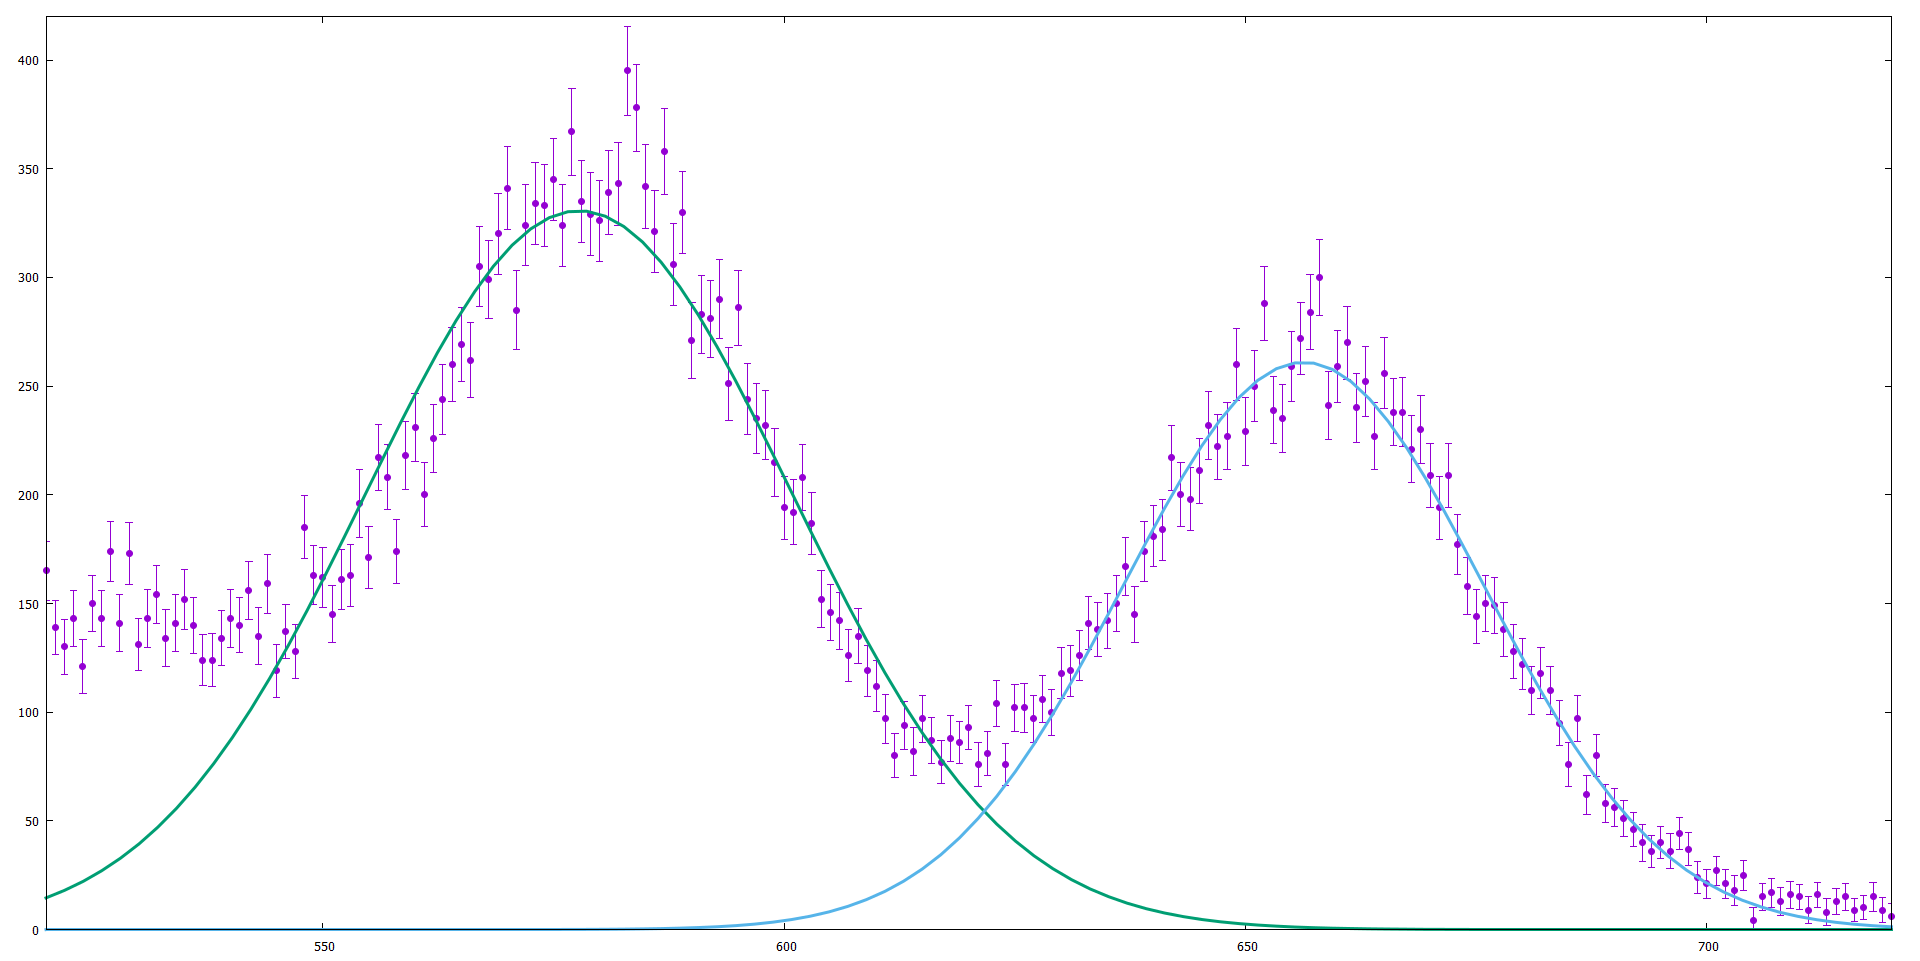
\includegraphics[width=8cm, height=5cm ]{rap14rys5} 
\caption{Krzywa dopasowania: piki kobaltu.}
\end{minipage}
\end{figure}
\begin{figure}[h!]
\centering
\begin{minipage}{0.5\textwidth}
  \centering
  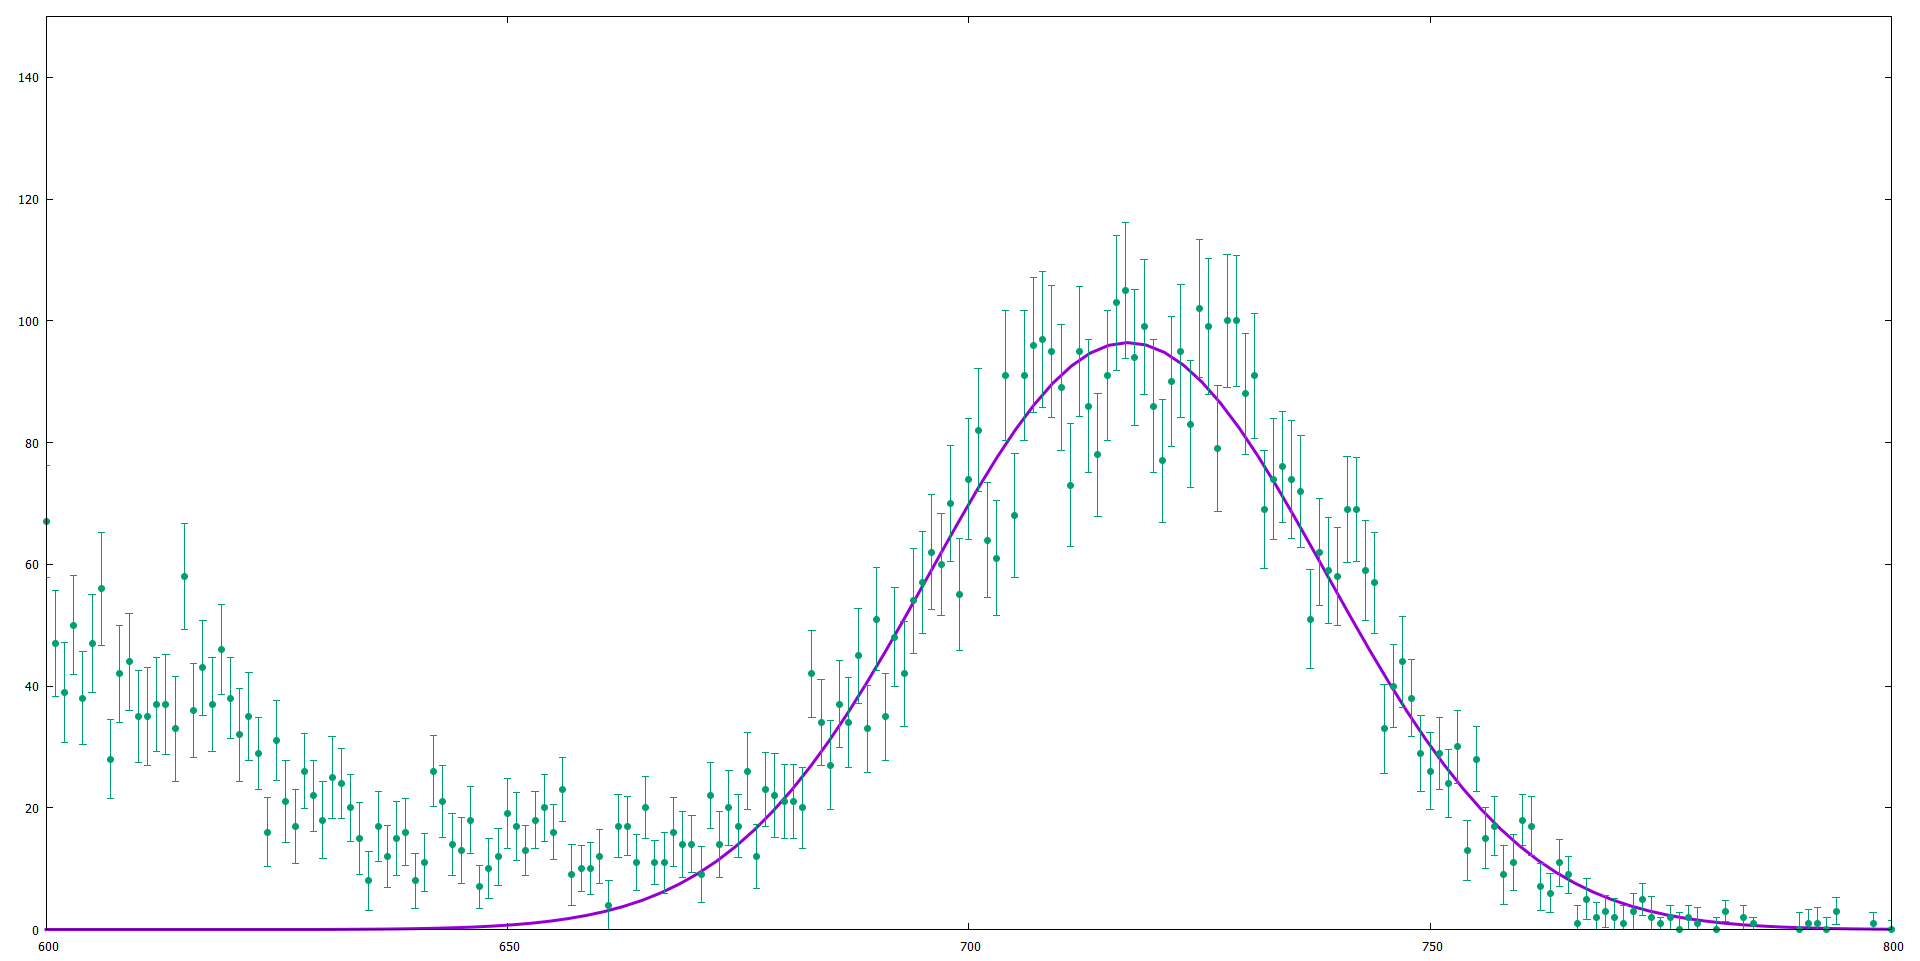
\includegraphics[width=8cm, height=5cm ]{rap14rys6} 
\caption{Krzywa dopasowania: pik potasu.}
\end{minipage}%
\begin{minipage}{0.5\textwidth}
  \centering
  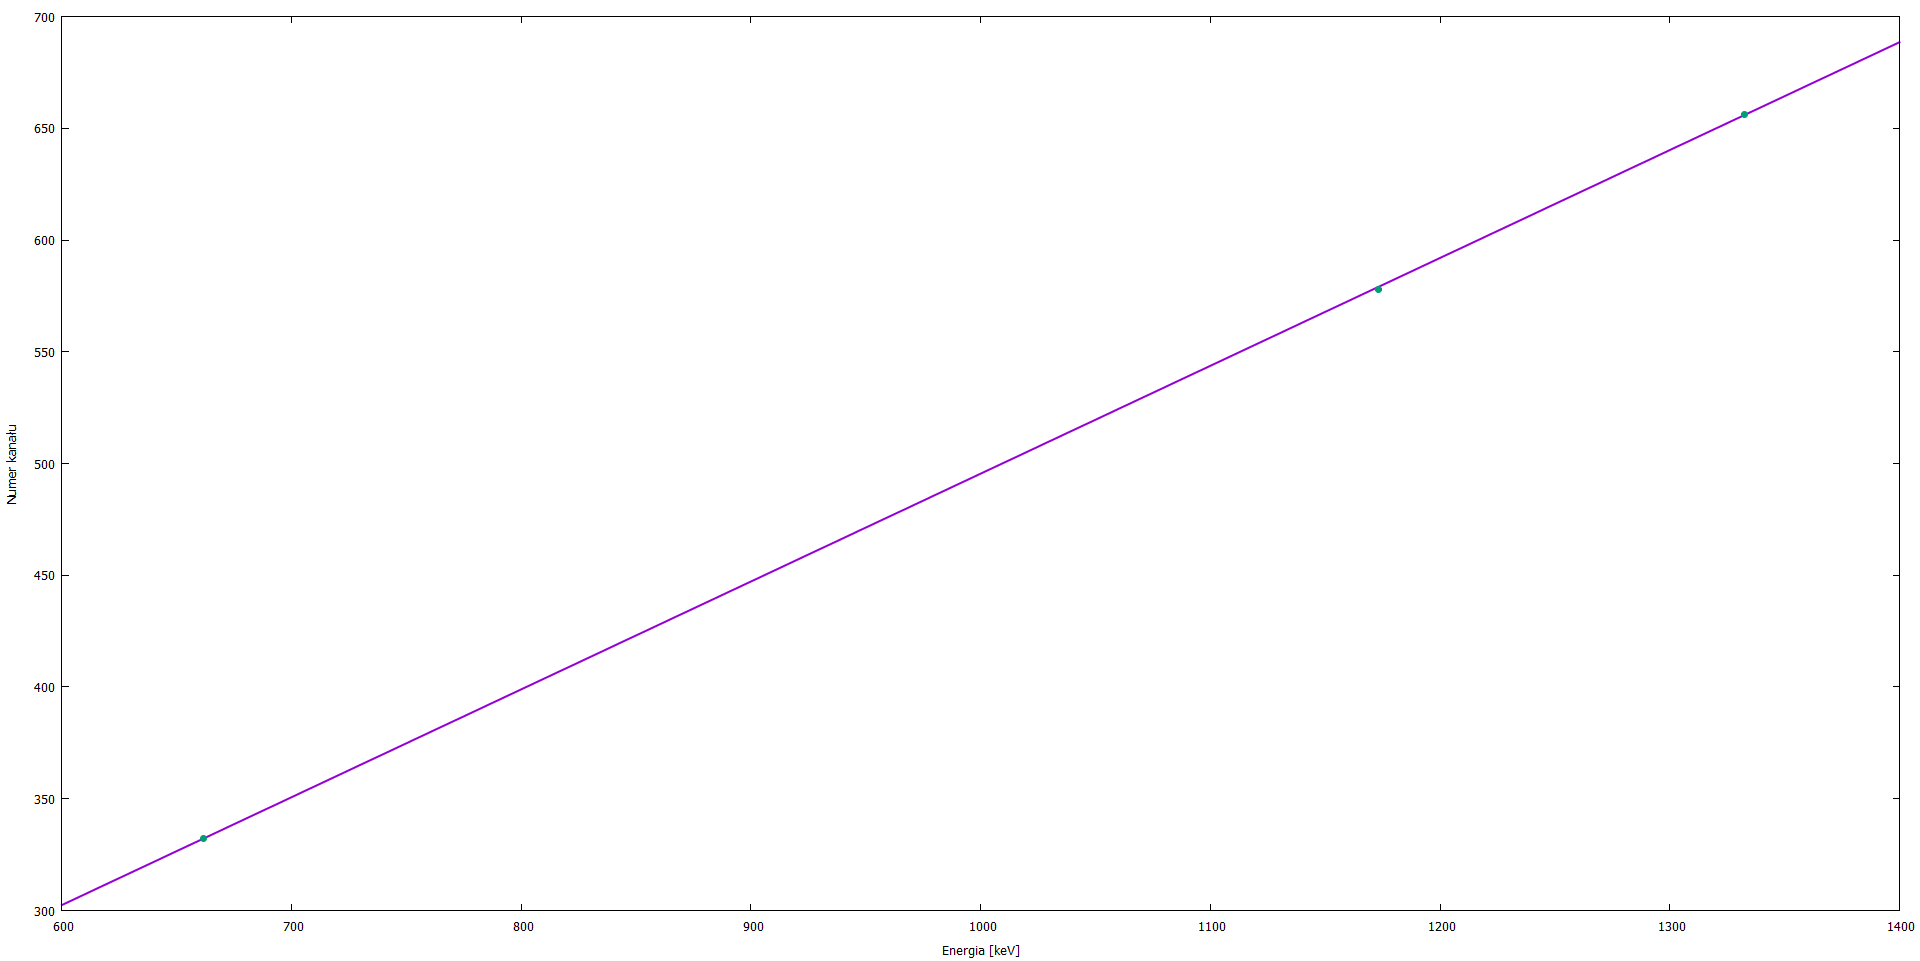
\includegraphics[width=8cm, height=5cm ]{rap14rys7} 
\caption{Krzywa zależności energii od kanału.}
\end{minipage}
\end{figure}


\begin{table}[h!]
\centering
\caption{Parametry dopasowania.}
\begin{tabular}{|c|c|c|c|c|c|c|c|}
\hline
\multicolumn{4}{|c|}{Cez}                  & \multicolumn{4}{c|}{Potas}               \\ \hline
Parametr    & $\sigma$  & $\mu$    & $N$   & Parametr   & $\sigma$ & $\mu$  & $N$     \\ \hline
Wartość     & 12,733    & 332,242  & 49955 & Wartość    & 21,50    & 717,25 & 5196,88 \\ \hline
Niepewność  & 0,067     & 0,075    & 271   & Niepewność & 0,35     & 0,40   & 87,72   \\ \hline
\multicolumn{4}{|c|}{Pierwszy pik kobaltu} & \multicolumn{4}{c|}{Drugi pik kobaltu}   \\ \hline
Wartość     & 23,12     & 577,75   & 19158 & Wartość    & 19,54    & 656,29 & 12780   \\ \hline
Niepewność  & 0,45      & 0,40     & 295   & Niepewność & 0,25     & 0,25   & 135     \\ \hline
\end{tabular}
\end{table}

Wartości $\mu$ wskazują na numer kanału, dla którego funkcja osiąga maksimum. Wartość tę można bezpośrednio powiązać z energią $E$ emitowanego kwantu $\gamma$, znając wartości energii dla cezu i kobaltu oraz wiedząc, że zależność między numerem kanału, a energią jest zależnością liniową. 

W Tabeli 2 przedstawiono wartości $\mu$, jej niepewności oraz wartości energii opowiadające danemu rozpadowi $\gamma$. Do tych danych dopasowano krzywą postaci $\mu=aE+b$. W tej samej tabeli przedstawiono parametry najlepszego dopasowania tej krzywej. Samą krzywą wraz z punktami przedstawiona na Rysunku 8.


\begin{table}[h!]
\centering
\caption{Dane: zależność energii od kanału; parametry dopasowania prostej.}
\label{my-label}
\begin{tabular}{|c|c|c|c|}
\hline
Próbka                & Cez           & Kobalt 1         & Kobalt 2                \\ \hline
$\mu$                 & 332,242       & 577,75           & 656,29                  \\ \hline
Niepewność            & 0,075         & 0,40             & 0,25                    \\ \hline
Energia $E$ [keV]         & 661,7         & 1173,2           & 1332,5                  \\ \hline
Parametry dopasowania & Wartość [keV] & Niepewność [keV] & Kowariancja             \\ \hline
$a $                    & 0,4825        & 0,0013           & \multirow{2}{*}{-0,965} \\ \cline{1-3}
$b$                     & 12,94         & 0,96             &                         \\ \hline
\end{tabular}
\end{table}
Niestety wartość $\chi^2$ dla tej krzywej wynosi 12,73, która to jest znacznie większa od wartości krytycznej wynoszącej 3,84. Tak więc zależność między energią a numerem kanału nie jest zależnością liniowa. Mimo to postanowiono kontynuować analizę posługując się tą zależnością oraz wyznaczonymi parametrami.

Aby wyznaczyć energię $E$ przy znanym numerze kanału należy odwrócić zależność $\mu=aE+b$.  Tak więc $E=\mu/a -b/a$. Przy obliczaniu niepewności energii należy dodatkowo uwzględnić ocenę kowariancji między parametrami $a$ i $b$.

Wykorzystano odwróconą zależność do obliczenia wartości energii dla rozpadu $\gamma$ potasu. Niepewność obliczono przy pomocy Równania (5). Otrzymano wartość $E=1460\pm110$ keV, która jest zgodna z wartością rzeczywistą wynoszącą 1460,8 keV. 

Dodatkowo, na podstawie parametrów piku cezu wyznaczono energetyczną zdolność rozdzielczą spektrometru. Obliczono ją ze stosunku szerokości piku w połowie jego wysokości do położenia maksimum piku. Otrzymano wartość 9,024$\%$, którą to zaokrąglono do $9\%$.

Wiedząc, że wydajność rejestracji kwantów gamma wynosi $\eta=(0,086\pm0,005)\%$ jak i znając liczbę $N$ przypadków pełnej absorpcji oraz to, że rozpad $\gamma$ następuje tylko w 11$\%$ przypadków obliczono początkową liczbę $N_{0}$ atomów potasu $^{40}$K. Skorzystano z danych z Tabeli 1 oraz z Równania (1), Równania (2) jak i z Równania (5), by obliczyć niepewność. Otrzymano wartość $N_{0}=(17,48\pm1,06)\cdot10^{20}$. Znając tę wartość, można podstawić ją do Równania (3) oraz Równania (4) przyjmując wartości $m_{39}=39,1$ g/mol, $m_{40}=40,0$ g/mol, $m_{s}=138,2$ g/mol, $N_{A}=6,022\cdot10^{23}$ 1/mol oraz $M=1011,91$ g. Zakładając, że wszystkie te wartości są znane dokładnie, otrzymano:
$M_{40}=0,1161\pm0,0070$ g, $M_{39}=572,4723\pm0,0069$ g. Tak więc stosunek $s=M_{40}/(M_{39}+M_{40})$ wynosi $s=(0,0203\pm0,0012)\%$. Wartość ta nie jest zgodna z wartością rzeczywistą, która wynosi $0,0117\%$. 

Aby dopełnić analizę potasu $^{40}$K postanowiono obliczyć aktywność badanej próbki. Otrzymano wartość $A=30500\pm1847$ Bq.


\begin{center}
\textbf{\subsection*{DYSKUSJA WYNIKÓW I WNIOSKI}}
\end{center} 
Otrzymana wartość $s$ choć niezgodna z wartością rzeczywistą, daje poprawne oszacowanie rzędu wielkości szukanego stosunku. Samą niezgodność wyników można usprawiedliwić tym, iż wykorzystywany spektrometr był uszkodzony i nie mierzył poprawnie liczby rozpadów. Jednakże otrzymane informacje mówiły o tym, iż otrzymane wartości powinny być dwukrotnie niższe od rzeczywistych, tymczasem jak się okazuje, błąd następuje w drugą stronę: otrzymane wartości są dwukrotnie wyższe. Aby rozstrzygnąć tę kwestię, należałyby sprawdzić spektrometr przy pomocy znanego źródła i skorygować ten błąd.
\begin{center}
\begin{thebibliography}{9}

 
\bibitem{tay1}
 J. R. Taylor,
 \emph{Wstęp do analizy błędu pomiarowego},
 PWN, Warszawa, 1995, s. 175.
 
 

 \end{thebibliography}

\end{center}


\end{document}